% !TEX encoding = UTF-8 Unicode
% !TEX root = ../../relatorio.tex

%% Responsavel:

\subsection{Questão 3.8}

Suppose \texttt{comm\_sz = 8} and \texttt{n = 16}.

a. Draw a diagram that shows how MPI Scatter can be implemented using
tree-structured communication with \texttt{comm\_sz} processes when process 0 needs to distribute an array containing n elements.

b. Draw a diagram that shows how MPI Gather can be implemented using
tree-structured communication when an n-element array that has been distributed among \texttt{comm\_sz} processes needs to be gathered onto process 0.\\

\begin{figure}[h!]
  \begin{center}
    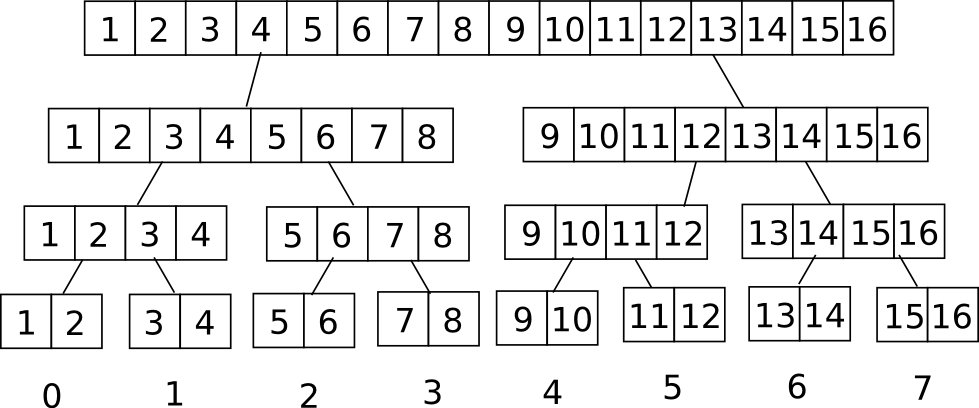
\includegraphics[width=290pt]{sections/q3.8/imgs/g1.png}
  \end{center}
  \caption{Scatter em comunição baseada em árvore}
  \label{fig:scattertree}
\end{figure}

\begin{figure}[h!]
  \begin{center}
    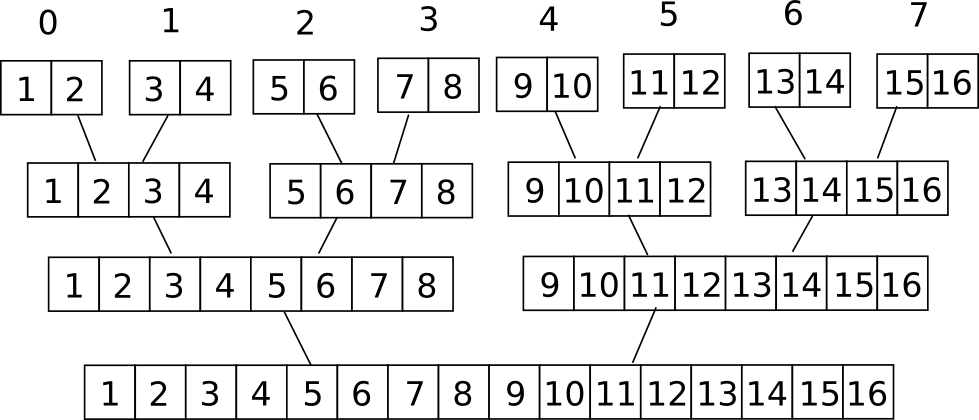
\includegraphics[width=290pt]{sections/q3.8/imgs/g2.png}
  \end{center}
  \caption{Gather em comunição baseada em árvore}
  \label{fig:gathertree}
\end{figure}




%%% Local Variables:
%%% mode: latex
%%% TeX-master: "../../relatorio"
%%% End:
